\section{Inverse funktioner, logaritme- og eksponentialfunktioner samt trigonometriske funktioner}
\begin{enumerate}
	\item Udregn følgende tal
	\begin{align*}
	3^3,&& 2^{-1}, &&\Big(\frac{1}{-1}\Big)^{3},&&\Big(\frac{1}{2}\Big)^{-3},&& 123^0.
	\end{align*}
	\item Udregn følgende tal
	\begin{align*}
	\log_2(128),&& \log_{10}(100),&& \log_5\Big(\frac{1}{25}\Big),&& \ln(e^3),&&\log_{123}(1).
	\end{align*}
	
	\item Udregn følgende tal
	\begin{align*}
	\sin(\frac{\pi}{4})+\cos(\frac{\pi}{4}),&& \tan(\frac{\pi}{3})+\cos(\frac{\pi}{6}),&& \frac{\sin(\frac{\pi}{6})+\cos(\frac{\pi}{3})}{\sin(\frac{2\pi}{3})}.
	\end{align*}
	

	\item Udregn følgende tal
	\begin{align*}
	\log_{10}(4)+\log_{10}(250),&&\log_{10}(25)-\log_{10}(5)+\log_{10}(2),&& \log_3(54)+\log_3\Big(\frac{1}{2}\Big)
	\end{align*}
	
	\item Udregn følgende
	\begin{align*}
	\cos(-\frac{5\pi}{4}),&& \sin(\frac{5\pi}{3}),&&\tan(-\frac{5\pi}{4}),&& \cos(\frac{8\pi}{3}).
	\end{align*}
	
	
	\item Reducer følgende
	\begin{align*}
	\ln(\sqrt{2})+\ln(2),&& \log_{10}(5^{3/2})+\frac{1}{2}\log_{10}(5)+\log_{10}(4),&& \frac{1}{4}\log_5(4^2+3^2).
	\end{align*}
	
	
	\item Udregn følgende tal
	\begin{align*}
	3^{\log_3(1)},&&e^{1+\ln(3)},&& 10^{-\log_{10}(7)},&& 7^{1-\log_7(9)},&& 4^{-\log_2(3)}.
	\end{align*}
	
	\item Udregn
	\begin{align*}
	\cos(\frac{13\pi}{3}),&& \tan(\frac{12\pi}{6}),&& \sin(-\frac{10\pi}{4}),&& \tan(\frac{15 \pi}{5}).
	\end{align*}
	
	
	\item Løs ligningerne 
	\begin{align*}
	e^x=3,&& \ln(x)=4,&& \ln(2x-4)=\ln(8)+\ln(4),&& 3\log_{10}(x)=\log_{10}(27).
	\end{align*}
	

	\item Bestem to forskellige løsninger til ligningerne 
	\begin{align*}
	\sin(x)=\frac{\sqrt{2}}{2},&& \cos(x-\pi)=-\frac{\sqrt{3}}{2},&& 2\cos^2(x)+5\cos(x)+2=0.
	\end{align*}

\item \label{it:trig3} I denne opgave beviser vi nogle af de eksakte værdier for sinus og cosinus til vinklerne $ \frac{\pi}{6}$ og $ \frac{\pi}{6} $.

\begin{enumerate}
	\item Vis at $\sin(\frac{\pi}{6})=\frac{1}{2}$ ved at regne på trekanten i Figur~\ref{fig:trig3}. (Hint: Hvad kan man sige om sidelængderne i trekanten?)
	
	\item Brug idiotformlen ($ \cos^2(x)+\sin^2(x)=1 $) til at vise at $\cos(\frac{\pi}{6})=\frac{\sqrt{3}}{2}$.
	
	\item Vis at $\sin(\frac{\pi}{3})=\frac{\sqrt{3}}{2}$. (Hint: $ \sin(\frac{\pi}{3})=\sin(\frac{\pi}{6}+\frac{\pi}{6})=2\sin(\frac{\pi}{6})\cos(\frac{\pi}{6}) $)
	
	\item Brug idiotformlen til at vise at $\cos(\frac{\pi}{3})=\frac{1}{2}$.
	
\end{enumerate}

\begin{figure}
	\centering
	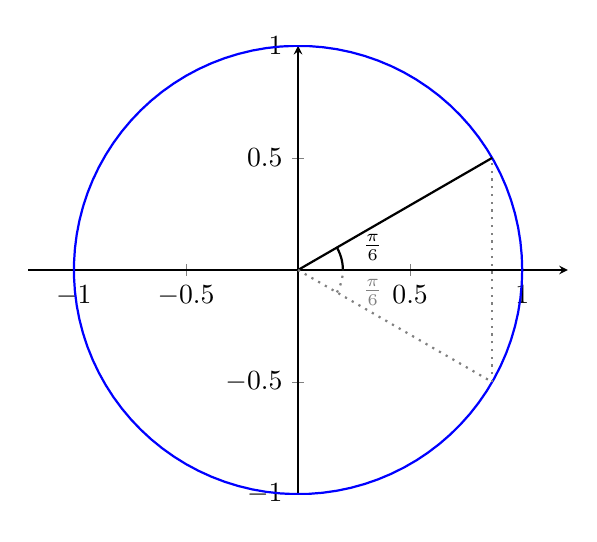
\begin{tikzpicture}
	\begin{axis}[xmin=-1,xmax=1,ymin=-1,ymax=1,axis x line=center,
	axis y line=center, axis equal]
	\addplot[blue,domain=0:2*pi,thick, samples=100] ({cos(deg(x))},{sin(deg(x))});
	\addplot[domain=0:sqrt(3)/2,thick] {1/sqrt(3)*x};
	\addplot[domain=0:pi/6,thick,samples=100] ({0.2*cos(deg(x))},{0.2*sin(deg(x))}) node[label={[label distance=2pt]0.5:\small$\frac{\pi}{6}$},pos=1] {};
	\addplot[domain=0:sqrt(3)/2,thick,gray,dotted] {-1/sqrt(3)*x};
	\addplot[domain=-pi/6:0,thick,samples=100,gray,dotted] ({0.2*cos(deg(x))},{0.2*sin(deg(x))}) node[label={[label distance=2pt]0.5:\small$\frac{\pi}{6}$},pos=0] {};
	\addplot[dotted,gray,thick] coordinates {(sqrt(3)/2, -1/2) (sqrt(3)/2, 1/2)};
	\end{axis}
	\end{tikzpicture}
	\caption{Opgave~\ref{it:trig3}}
	\label{fig:trig3}
\end{figure}

\item \label{it:trig4} I denne opgave beviser vi nogle af de eksakte værdier for sinus og cosinus til vinklen $ \frac{\pi}{4}$.
\begin{enumerate}
	\item Vis at $\sin(\frac{\pi}{4})=\frac{\sqrt{2}}{2}$ ved at regne på trekanten i Figur~\ref{fig:trig4}.(Hint: Pythagoras) 
	\item Brug idiotformlen til at vise at $\cos(\frac{\pi}{4})=\frac{\sqrt{2}}{2}$. 
\end{enumerate}

\begin{figure}
	\centering
	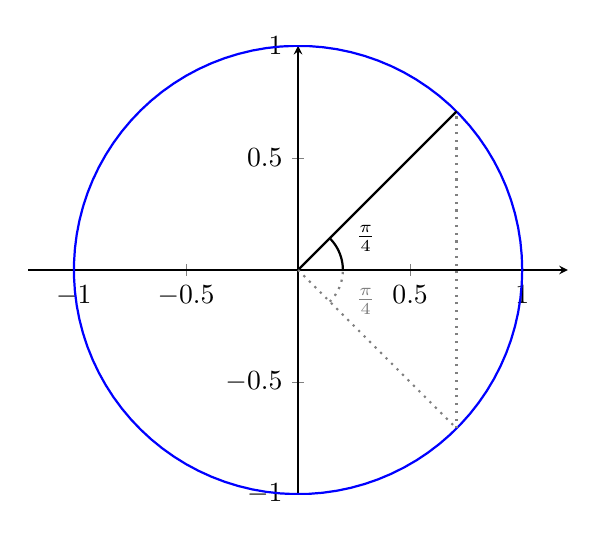
\begin{tikzpicture}
	\begin{axis}[xmin=-1,xmax=1,ymin=-1,ymax=1,axis x line=center,
	axis y line=center, axis equal]
	\addplot[blue,domain=0:2*pi,thick, samples=100] ({cos(deg(x))},{sin(deg(x))});
	\addplot[domain=0:sqrt(2)/2,thick] {1*x};
	\addplot[domain=0:pi/4,thick,samples=100] ({0.2*cos(deg(x))},{0.2*sin(deg(x))}) node[label={[label distance=2pt]0.5:\small$\frac{\pi}{4}$},pos=1] {};
	\addplot[domain=0:sqrt(2)/2,thick,gray,dotted] {-1*x};
	\addplot[domain=-pi/4:0,thick,samples=100,gray,dotted] ({0.2*cos(deg(x))},{0.2*sin(deg(x))}) node[label={[label distance=2pt]0.5:\small$\frac{\pi}{4}$},pos=0] {};
	\addplot[dotted,gray,thick] coordinates {({sqrt(2)/2}, -{sqrt(2)/2}) ({sqrt(2)/2}, {sqrt(2)/2})};
	\end{axis}
	\end{tikzpicture}
	\caption{Opgave~\ref{it:trig4}}
	\label{fig:trig4}
\end{figure}

\end{enumerate}